%
% trigonometrisch.tex
%
% (c) 2021 Prof Dr Andreas Müller, OST Ostschweizer Fachhochschule
%
\section{Trigonometrische Funktionen
\label{buch:geometrie:section:trigonometrisch}}
\rhead{Trigonometrische Funktionen}
Die Navigation zur See wie auch die Landvermessung hängen davon ab,
dass man Winkel zwischen Himmelskörpern, Landmarken oder dem Horizont
messen kann.
Aus solchen Messungen können dann mittels bekannter Beziehungen
zwischen den Winkeln und Seitenlängen in Dreiecken weitere Seitenlängen
und Winkel berechnet werden.
Schon in rechtwinkligen Dreiecken sind die Beziehungen zwischen Winkel
und Seitenlängen von einer Art, die sich nicht durch algebraische
Ausdrücke berechnen lässt.
Es ist daher notwendig, neue spezielle Funktionen zu definieren,
die trigonometrischen Funktionen.

%
% Definition der trigonometrischen Funktionen
%
\subsection{Definition der trigonometrischen Funktionen}
% XXX Abbildung Jakobsstab
Eines der ältesten Messgeräte für Winkel ist der Jakobsstab,
dargestellt in Abbildung~\ref{}.
Der Querstab kann entlang des Stabs verschoben werden.
Die beiden Punkte, deren Zwischenwinkel bestimmt werden soll,
werden so anvisiert, dass sie sich auf den Enden des Querstabs 
zu befinden scheinen.
Abgelesen wird dann die Strecke $l$ zwischen dem Auge des Beobachters
und dem Querstab.
Daraus und aus der Länge $l_Q$ des Querstabes lässt sich jetzt der Winkel
mit der Formel
\[
\tan\frac{\alpha}2 = \frac{l_Q}{2l}
\]
berechnen.
Um nun einen numerischen Wert für $\alpha$ zu bekommen, braucht man
eine Tabelle der Funktionswerte der Funktion auf der linken Seite.

\begin{figure}
\centering
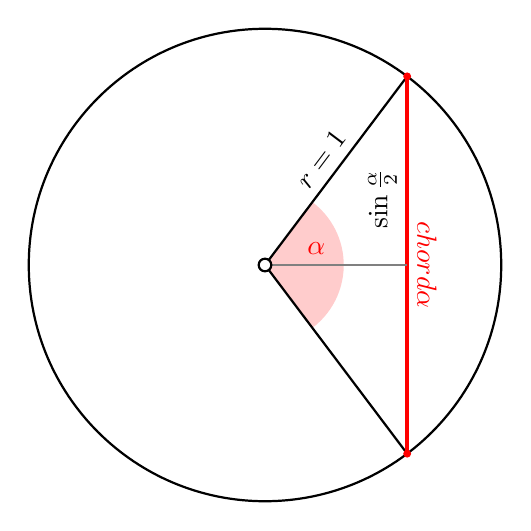
\begin{tikzpicture}[>=latex,thick]
\def\r{3}
\def\a{53}
\fill[color=red!20] (0,0) -- (-\a:1) arc (-\a:\a:1) -- cycle;
\draw (0,0) -- (\a:\r);
\draw (0,0) -- (-\a:\r);
\node[color=red] at ({cos(\a/2)},0) [above left] {$\alpha$};
\draw (0,0) circle[radius=\r];
\draw[color=red,line width=1.4pt] (\a:\r) -- (-\a:\r);
\fill[color=red] (\a:\r) circle[radius=0.05];
\fill[color=red] (-\a:\r) circle[radius=0.05];
\node[color=red] at ({\r*cos(\a)},0)
	[above,rotate=-90] {$\operatorname{chord}\alpha$};
\draw[color=gray,line width=1.0pt] (0,0) -- ({\r*cos(\a)},0);
\fill[color=white] (0,0) circle[radius=0.08];
\draw (0,0) circle[radius=0.08];
\node at (\a:{0.5*\r}) [above,rotate=\a] {$r=1$};
\node at ({\r*cos(\a)},{0.35*\r*sin(\a)})
	[above,rotate=90] {$\sin\frac{\alpha}2$};
\end{tikzpicture}
\caption{Definition der Chord-Funktion $\operatorname{chord}\alpha$
am Einheitskreis.
\label{buch:geometrie:trigo:chorddef}}
\end{figure}

Die älteste bekannt Tabelle von Funktionswerten trigonometrischer
Funktionen stammt von Hipparchus aus dem 2.~Jahrhundert BCE und
enthält Werte der sogenannten Chord-Funktion $\operatorname{chord}\alpha$,
welche die Länge der Sehne eines Bogens $\alpha$ des Einheitskreises
berechnet.
Aus der Abbildung~\ref{buch:geometrie:trigo:chorddef} ergibt sich
\[
\operatorname{chord}\alpha = 2\sin\frac{\alpha}2.
\]
Die Verwendung der Chord-Funktion war bis ins 19.~Jahrhundert in der
Landvermessung üblich.
Neben der Chord-Funktion waren auch noch andere heute weitgehend
vergessen Funktionen im Einsatz wie zum Beispiel der Sinus versus
\[
\operatorname{vers}\alpha=1-\cos\alpha
=
2\sin^2\frac{\alpha}2
\]
oder der Semiversus
\[
\operatorname{sem}\alpha
=
\frac{\operatorname{vers}\alpha}{2}
=
\sin^2\frac{\alpha}2,
\]
der besonders nützlich bei der Berechnung der Entfernung
zweier in geographischer Länge und Breite gegebener Punkte
auf der Erdoberfläche ist und daher in der Navigation lange
üblich war.

Eine neue spezielle Funktion sollte sowohl möglichst
universell einsetzbar sein als auch gut und effizient
berechnet werden können.
Aus dieser Forderung haben sich die Funktion $\sin\alpha$,
$\cos\alpha$ und $\tan\alpha$ als die nützlichsten herausgestellt.
Mit ihnen lassen sich a

%
% Rechtwinklige Dreiecke
%
\subsubsection{Rechtwinklige Dreiecke}
Ähnliche Dreiecke haben gleiche Seitenverhältnisse und Winkel.
Rechtwinklige Dreiecke sind daher bis auf Ähnlichkeit vollständig
durch die Angabe eines Winkels beschrieben.
Die Seitenverhältnisse müssen daher aus den Winkeln berechnet werden
können.
Genau dies ist die Aufgabe, die die trigonometrischen Funktionen lösen.

\begin{figure}
\centering
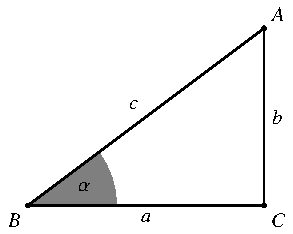
\includegraphics{chapters/030-geometrie/images/deftrig.pdf}
\caption{Rechtwinkliges Dreieck zur Definition der trigonometrischen
Funktionen.
\label{buch:geometrie:trigo:fig:definition}}
\end{figure}

\begin{definition}
\label{buch:geometrie:def:trigo}
In einem rechtwinkligen Dreieck mit Winkel $\alpha$, $0<\alpha < \frac{\pi}2$,
sind die Seitenverhältnisse gegeben durch die trigonometrischen Funktionen,
die wie folgt definiert sind:
\begin{align*}
\sin\alpha &= \frac{\text{Gegenkatete}}{\text{Hypothenuse}} = \frac{b}{c},
&
\cos\alpha &= \frac{\text{Ankatete}}{\text{Hypothenuse}} = \frac{a}{c}
&&\text{und}
&
\tan\alpha &= \frac{\text{Gegenkatete}}{\text{Ankatete}} = \frac{a}{b}
\intertext{mit den Kehrwerten}
\sec\alpha &= \frac{\text{Hypothenuse}}{\text{Gegenkatete}} = \frac{c}{b},
&
\csc\alpha &= \frac{\text{Hypothenuse}}{\text{Ankatete}} = \frac{c}{a}
&&\text{und}
&
\cot\alpha &= \frac{\text{Ankatete}}{\text{Gegenkatete}} = \frac{b}{a}
\end{align*}
(siehe auch Abbildung~\ref{buch:geometrie:trigo:fig:definition}).
\end{definition}

Aus der Definition und dem Satz von Pythagoras kann eine grosse Zahl
von Beziehungen zwischen den trigonometrischen Funktionen abgeleitet
werden.
Zum Beispiel folgt sofort
\[
\sin^2\alpha+\cos^2\alpha
=
\biggl(\frac{b}{c}\biggr)^2
+
\biggl(\frac{a}{c}\biggr)^2
=
\frac{a^2+b^2}{c^2} 
=
1.
\]
Insbesondere lässt sich $\sin\alpha$ durch $\cos\alpha$ ausdrücken
und umgekehrt:
\[
\sin\alpha
=
\sqrt{1-\cos^2\alpha\mathstrut}
\qquad\text{und}\qquad
\cos\alpha
=
\sqrt{1-\sin^2\alpha\mathstrut}
\]
Da sich alle Funktionen durch $\cos\alpha$ und $\sin\alpha$ ausdrücken
lassen, können alle auch nur durch eine ausgedrückt werden.
Durch Umkehrung dieser Beziehung kann man jede der trigonometrischen
Funktionen durch jede andere ausdrücken, wie dies in
Tabelle~\ref{buch:geometrie:tab:trigo} zusammengestellt ist.

\begin{figure}
\centering
\renewcommand{\arraystretch}{2.5}
\renewcommand{\tabcolsep}{5pt}
\begin{tabular}{|>{$}c<{$}|>{$}c<{$}>{$}c<{$}>{$}c<{$}>{$}c<{$}>{$}c<{$}>{$}c<{$}|}
\hline
%\downarrow\text{ ausgedrückt durch }\rightarrow
&\sin\alpha&\cos\alpha&\tan\alpha&\cot\alpha&\sec\alpha&\csc\alpha\\[5pt]
\hline
\sin\alpha
	&\sin\alpha
	&\sqrt{1-\cos^2\alpha\mathstrut}
		&\displaystyle\frac{\tan\alpha}{\sqrt{1+\tan^2\alpha}}
		&\displaystyle\frac{1}{\sqrt{1+\cot^2\alpha}}
			&\displaystyle\frac{1}{\sec\alpha}
			&\displaystyle\frac{\sqrt{\csc^2\alpha-1}}{\csc\alpha}
\\
\cos\alpha
	&\sqrt{1-\sin^2\alpha\mathstrut}
	&\cos\alpha
		&\displaystyle\frac{1}{\sqrt{1+\tan^2\alpha}}
		&\displaystyle\frac{\cot\alpha}{\sqrt{1+\cot^2\alpha}}
			&\displaystyle\frac{\sqrt{\sec^2\alpha-1}}{\sec\alpha}
			&\displaystyle\frac{1}{\csc\alpha}
\\
\tan\alpha
	&\displaystyle\frac{\sin\alpha}{\sqrt{1-\sin^2\alpha\mathstrut}}
	&\displaystyle\frac{\sqrt{1-\cos^2\alpha\mathstrut}}{\cos\alpha}
		&\tan\alpha
		&\displaystyle\frac{1}{\cot\alpha}
			&\displaystyle\frac{1}{\sqrt{\sec^2\alpha-1}}
			&\displaystyle\sqrt{\csc^2\alpha-1}
\\
\cot\alpha
	&\displaystyle\frac{\sqrt{1-\sin^2\alpha\mathstrut}}{\sin\alpha}
	&\displaystyle\frac{\cos\alpha}{\sqrt{1-\cos^2\alpha\mathstrut}}
		&\displaystyle\frac{1}{\tan\alpha}
		&\cot\alpha
			&\displaystyle\sqrt{\sec^2\alpha-1}
			&\displaystyle\frac{1}{\sqrt{\sec^2\alpha-1}}
\\
\sec\alpha
	&\displaystyle\frac{1}{\sin\alpha}
	&\displaystyle\frac{1}{\sqrt{1-\cos^2\alpha\mathstrut}}
		&\displaystyle\frac{\sqrt{1+\tan^2\alpha}}{\tan\alpha}
		&\displaystyle\sqrt{1+\cot^2\alpha}
			&\sec\alpha
			&\displaystyle\frac{\csc\alpha}{\sqrt{\csc^2\alpha-1}}
\\
\csc\alpha
	&\displaystyle\frac{1}{\sqrt{1-\sin^2\alpha\mathstrut}}
	&\displaystyle\frac{1}{\cos\alpha}
		&\displaystyle\sqrt{1+\tan^2\alpha}
		&\displaystyle\frac{\sqrt{1+\cot^2\alpha}}{\cot\alpha}
			&\displaystyle\frac{\sec\alpha}{\sqrt{\sec^2\alpha-1}}
			&\csc\alpha
\\[8pt]
\hline
\end{tabular}
\caption{Darstellung aller trigonometrischen Funktionen durch jede beliebige
andere Funktion.
Für Winkel ausserhalb des 1.~Quadranten müssen die Vorzeichen der
Quadratwurzeln so gewählt werden, dass die Funktion das richtige
Vorzeichen erhält.
\label{buch:geometrie:tab:trigo}}
\end{figure}

Diese Definition~\ref{buch:geometrie:def:trigo}
ist auf spitze Winkel und damit auf nichtnegative Werte der
trigonometrischen Funktionen beschränkt.

%
% Definition am Einheitskreis
%
\subsubsection{Einheitskreis}
Im vorangegangen Abschnitt wurden die rechtwinkligen Dreiecke durch
einen Winkel charakterisiert und die trigonometrischen
Funktionen als Verhältnis von Seiten des Dreiecks abgeleitet.
Dabei wurde die Schwierigkeit übergangen, wie überhaupt der Winkel
definiert werden soll.
Ein Winkel war im Wesentlichen durch die Eigenschaft
definiert, dass ähnliche Dreiecke den gleichen Winkel haben.
Die Definition~\ref{buch:geometrie:def:trigo} ist in diesem Licht
nichts anderes als eine Namenskonvention für die Seitenverhältnisse
einer Klasse von ähnlichen rechtwinkligen Dreiecken.

\begin{figure}
\centering
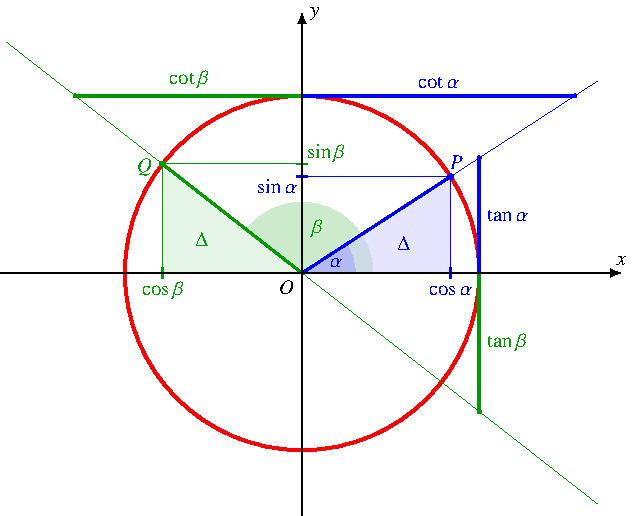
\includegraphics{chapters/030-geometrie/images/einheitskreis.pdf}
\caption{Definition der trigonometrischen Funktion mit Hilfe des
Einheitskreises
\label{buch:geometrie:trigo:fig:einheitskreis}}
\end{figure}

Eine alternative Charakterisierung rechtwinkliger Dreiecke
geht von Punkten auf dem Einheitskreis aus.
Die Lote von einem Punkt $P$ auf dem Einheitskreis definieren
zwei ähnliche Dreiecke, mit dem Ursprung $O$, dem Punkt $P$
und dem Fusspunkt des Lotes.
Die Koordinaten des Punktes $P$ können im Gegensatz zu den Seiten
des rechtwinkligen Dreiecks in
Abbildung~\ref{buch:geometrie:trigo:fig:definition}
auch negativ sein.
Ein Punkt im zweiten Quadranten hat zum Beispiel eine negative
$x$-Koordinate.
Die trigonometrischen Funktionen können nun analog zu
Definition~\ref{buch:geometrie:def:trigo} aber unter Verwendung
der Koordinaten $x$ und $y$.

Auch das Argument $\alpha$ der trigonometrischen Funktionen kann
jetzt auf natürlichere Art und Weise definiert werden.
Es ist die Länge des Bogens auf dem Einheitskreis zwischen dem
Punkt $(1,0)$ und $P$.
Damit lassen sich die trigonometrischen Funktionen jetzt
für beliebige Winkel $\alpha\in\mathbb{R}$ definieren.

\begin{definition}
\label{buch:geometrie:def:trigeinheitskreis}
Die trigonometrischen Funktionen des Winkels $\alpha$ zwischen der 
$x$-Achse und der Richtung durch den Punkt $P$ sind 
\begin{align*}
\sin\alpha &= x, &\cos\alpha &= y&&\text{und}& \tan\alpha=\frac{y}{x}
\intertext{mit den Kehrwerten}
\sec\alpha &= \frac{1}{x}, &\csc\alpha &= \frac{1}{y}&&\text{und}& \tan\alpha=\frac{x}{y}.
\end{align*}
(siehe auch Abbildung~\ref{buch:geometrie:trigo:fig:einheitskreis}).
\end{definition}

Die Beziehungen der Tabelle~\ref{buch:geometrie:tab:trigo}
zwischen den trigonometrischen Funktionen bleibt auch für 
diese erweiterten Funktionen gültig, wenn das Vorzeichen der
Quadratwurzel falls vorhanden geeignet gewählt wird.

%
% Drehungen in der Ebene
%
\subsection{Drehungen der Ebene}
Die Funktionen $\sin\alpha$ und $\cos\alpha$ sind in den Anwendungen
besonders nützlich, weil sich damit die Kreisbewegung parametrisieren
lässt.
Etwas allgemeiner kann man damit Drehungen der Ebene beschreiben.
Damit entstehen die Funktion als Nebenprodukt einer Parametrisierung
der Drehgruppe $\operatorname{SO}(2)$.
Daraus werden sich später Ableitungseigenschaften und
Potenzreihendarstellungen der trigonometrischen Funktionen ableiten
lassen.

\subsubsection{Drehmatrizen und Additionstheoreme}
Eine Drehung der Ebenen $\mathbb{R}^2$ um den Winkel $\alpha$ bildet
die Standardbasisvektoren auf die Vektoren
\[
e_1=\begin{pmatrix}1\\0\end{pmatrix}
\mapsto
\begin{pmatrix}
\cos\alpha\\\sin\alpha
\end{pmatrix}
\qquad\text{und}\qquad
e_2=\begin{pmatrix}0\\1\end{pmatrix}
\mapsto
\begin{pmatrix}
-\sin\alpha
\\
\cos\alpha
\end{pmatrix}
\]
ab.
Die Abildungsmatrix der Drehung ist daher
\[
D_\alpha
=
\begin{pmatrix*}[r]
\cos\alpha&-\sin\alpha\\
\sin\alpha& \cos\alpha
\end{pmatrix*}.
\]
Die Zusammensetzung zweier Drehungen um die Winkel $\alpha$ und $\beta$
ist wieder eine Drehung um den Winkel $\alpha+\beta$, es gilt
also
\[
D_{\alpha+\beta}
=
D_{\alpha}D_{\beta},
\]
oder in Matrizenform
\begin{align*}
D_{\alpha+\beta}
&=
\begin{pmatrix*}[r]
\cos(\alpha+\beta)&-\sin(\alpha+\beta) \\
\sin(\alpha+\beta)& \cos(\alpha+\beta)
\end{pmatrix*}
\\
=
D_{\alpha}D_{\beta}
&=
\begin{pmatrix*}[r]
\cos\alpha&-\sin\alpha\\
\sin\alpha&\cos\alpha
\end{pmatrix*}
\begin{pmatrix*}[r]
\cos\beta&-\sin\beta\\
\sin\beta&\cos\beta
\end{pmatrix*}
\\
&=
\begin{pmatrix}
\cos\alpha\cos\beta-\sin\alpha\sin\beta
	& -\cos\alpha\sin\beta -\sin\alpha\cos\beta\\\
\cos\alpha\sin\beta+\sin\alpha\cos\beta
	& \cos\alpha\cos\beta-\sin\alpha\sin\beta
\end{pmatrix}
\end{align*}
Aus dem Vergleich der beiden Matrizen liest man die Additionstheoreme.

\begin{satz}
Für $\alpha,\beta\in\mathbb{R}$ gilt
\begin{align*}
\sin(\alpha\pm\beta)
&=
\cos\alpha\cos\beta\mp\sin\alpha\sin\beta
\\
\cos(\alpha\pm\beta)
&=
\cos\alpha\cos\beta\pm\sin\alpha\sin\beta
\end{align*}
\end{satz}

Ein besonders einfacher Spezialfalls ist $\alpha=\beta$, es ergben sich die
Doppelwinkelformeln
\begin{align*}
\cos2\alpha &= \cos^2\alpha-\sin^2\alpha
\\
\sin2\alpha &= 2\cos\alpha\sin\alpha.
\end{align*}
In der Formel für $\cos2\alpha$ kann die rechte Seite durch nur
eine Winkelfunktion ausdrücken:
\begin{align*}
\cos2\alpha &= \cos^2\alpha - (1-\cos^2\alpha) = 2\cos^2\alpha -1
\\
\cos2\alpha &= (1-\sin^2\alpha) - \sin^2\alpha = 1-2\sin^2\alpha.
\end{align*}
Beide Ausdrücke lassen sich leicht nach den Funktionen auf der rechten
Seite auflösen, so erhält man die Halbwinkelformeln
\begin{align*}
\cos^2\alpha &= \frac{1+\cos2\alpha}2
&&\Rightarrow&
\cos^2\frac{\alpha}2 &=\frac{1+\cos\alpha}2
\\
\sin^2\alpha &= \frac{1-\cos2\alpha}2
&&\Rightarrow&
\sin^2\frac{\alpha}2 &= \frac{1-\cos\alpha}2.
\end{align*}
Der letzte Ausdruck ist auch bekannt als der Semiversus.

\subsubsection{Funktionen für mehrfache Winkel}
Die Additionstheoreme können dazu verwendet werden, Formeln für
die Werte der trigonometrischen Funktionen mehrfacher Winkel zu
finden.
Die Berechnung kann etwas vereinfacht werden, wenn man die Drehmatrix
mit Hilfe der Matrix
\[
J=\begin{pmatrix}0&-1\\1&0\end{pmatrix}
\]
als
\[
D_{\alpha}
=
E
\cos\alpha
+
J
\sin\alpha
\]
schreiben.
Die Potenzen von $J$ sind
\[
J^2 = -E,\quad
J^3 = -J \quad\text{und}\quad
J^4 = E.
\]
Daraus ergibt sich
\begin{align*}
D_{n\alpha}
=
(D_{\alpha})^n
&=
(E\cos\alpha+J\sin\alpha)^n
\\
&=
\sum_{k=0}^n \binom{n}{k}\cos^{n-k}\alpha\sin^{k}\alpha J^k
\\
&=
\sum_{l=0}^{\lfloor\frac{n}2\rfloor}
(-1)^l
\binom{n}{2l}\cos^{n-2l}\alpha \sin^{2l}\alpha 
-
J
\sum_{l=0}^{\lfloor\frac{n}2\rfloor}
(-1)^l
\binom{n}{2l+1}\cos^{n-2l-1}\alpha \sin^{2l+1}\alpha 
\intertext{Durch Vergleich mit der Matrix $D_{n\alpha}$ findet man die
Formeln für die Funktionen des $n$-fachen Winkels:}
\cos n\alpha
&=
\sum_{l=0}^{\lfloor\frac{n}2\rfloor}
(-1)^l
\binom{n}{2l}\cos^{n-2l}\alpha \sin^{2l}\alpha 
\\
\sin n\alpha
&=
-
\sum_{l=0}^{\lfloor\frac{n}2\rfloor}
(-1)^l
\binom{n}{2l+1}\cos^{n-2l-1}\alpha \sin^{2l+1}\alpha 
\end{align*}
Für kleine Werte von $n$ sind die Formeln einigermassen übersichtlich,
zum Beispiel für $n=3$:
\begin{align*}
\cos 3\alpha
&=
\cos^3\alpha-3\cos\alpha\sin^2\alpha
=
\cos^3\alpha-3\cos\alpha(1-\cos^2\alpha)
\\
&=
4\cos^3\alpha-3\cos\alpha,
\\
\sin 3\alpha
&=
3\cos^2\alpha\sin\alpha
-
\sin^3\alpha
=
3(1-\sin^2\alpha)\sin\alpha-\sin^3\alpha
\\
&=
-4\sin^3\alpha
+3\sin\alpha.
\end{align*}
Indem man diese Formeln als kubische Gleichungen für die
Unbekannte $\cos\alpha$ bzw.~$\sin\alpha$ betrachtet, kann
man durch Lösung der Gleichung zum Beispiel mit der Formel von
Cardano 
% XXX Verweis auf die Formel von Cardano
zu gegebenen Werten von $\cos 3\alpha$ und $\sin 3 \alpha$
die Werte von $\cos\alpha$ und $\sin\alpha$ durch rein
algebraische Operationen bestimmen.

\subsection{Eine Tabelle der Werte der trigonometrischen Funktionen
aufstellen
\label{buch:trigo:subsection:tabelle}}
Die älteste Tabelle der Werte trigonometrischer Funktionen stammt aus der
Feder von Hipparcos aus dem zweiten Jahrhundert BCE.
Sie hatte eine Auflösung von $1^\circ$.
Wie kann man eine solche Tabelle mit den Mitteln der damaligen Zeit,
also insbesondere ganz ohne Dezimalbrüche, zusammenstellen?

Aus speziellen Dreiecken kann man die einige wenige bekannte Winkel
finden und die zugehörigen Werte der trigonemetrischen Funktionen
bestimmen.
In einem rechtwinklig gleichschenkligen Dreieck liest man
\[
\sin 45^\circ = \cos 45^\circ
\]
ab.
Ein gleichseitiges Dreieck erlaubt
\begin{align*}
\sin 30^\circ &= \frac{1}{2} &
\cos 30^\circ &= \frac{\sqrt{3}}{2}
\\
\sin 60^\circ &= \frac{\sqrt{3}}{2} &
\cos 60^\circ &= \frac{1}{2}
\intertext{zu bestimmen.
Mit Hilfe der Halbwinkelformeln werden daraus die Werte
von $15^\circ$:}
\sin 15^\circ &= \sqrt{\frac{2-\sqrt{3}}{4}} &
\cos 15^\circ &= \sqrt{\frac{2+\sqrt{3}}{4}}.
\end{align*}
Mit Hilfe der Additionstheoreme kann man jetzt auch noch die Werte
für den Winkel $75^\circ$ bestimmen.
Damit sind die Werte der Sinus- und Kosinus-Funktion für alle
Vielfachen von $15^\circ$ bekannt.

Etwas spezieller ist die Situation eines Fünfecks, welches den
Zentriwinkel $72^\circ$ hat, damit kann man die Werte 
\begin{align*}
\sin 36^\circ &=
\sqrt{\frac{5-\sqrt{5}}8}
&&\text{und}&
\cos 36^\circ &=
\sqrt{\frac{3+\sqrt{5}}{8}}
\\
\sin 72^\circ &=
2
\sqrt{\frac{5-\sqrt{5}}8}
\sqrt{\frac{3+\sqrt{5}}{8}}
=
\sqrt{5+\sqrt{5}}
&&&
\cos 72^\circ &=
\frac{3+\sqrt{5}}{8}
-
\frac{5-\sqrt{5}}{8}
=
\frac{-1+\sqrt{5}}{4}
\intertext{%
Mit den Halbwinkelformeln kann man dies nochmals teilen, bis man
die Winkel}
\sin 18^\circ &=
\sqrt{\frac12-\frac12
\sqrt{\frac{3+\sqrt{5}}{8}}
}
&&\text{und}&
\cos 18^\circ &=
\sqrt{\frac12+\frac12
\sqrt{\frac{3+\sqrt{5}}{8}}
}
\intertext{sowie}
\sin 9^\circ &=
\sqrt{\frac12-\frac12
\sqrt{\frac12+\frac12
\sqrt{\frac{3+\sqrt{5}}{8}}
}
}
&&\text{und}&
\cos 9^\circ &=
\sqrt{\frac12+\frac12
\sqrt{\frac12+\frac12
\sqrt{\frac{3+\sqrt{5}}{8}}
}
}
\end{align*}
ausgwertet hat.

\begin{table}
\centering
\begin{tabular}{|>{$}r<{$}>{$}c<{$}>{$}l<{$}|>{$}r<{$}>{$}c<{$}>{$}l<{$}|>{$}r<{$}|>{$}r<{$}|}
\hline
\alpha&&&90^\circ-\alpha&&&\sin\alpha&\cos\alpha\\
\hline
 0^\circ & &                   &          & &                  &0.00000000&1.00000000\\
 3^\circ &=&18^\circ-15^\circ  & 87^\circ &=&72^\circ+15^\circ &0.05233596&0.99862953\\
 6^\circ &=&15^\circ-\phantom{0}9^\circ   & 84^\circ &=&75^\circ+\phantom{0}9^\circ  &0.10452846&0.99452190\\
 9^\circ & &                   & 81^\circ &=&90^\circ-\phantom{0}9^\circ  &0.15643447&0.98768834\\
12^\circ &=&30^\circ-18^\circ  & 78^\circ &=&60^\circ+18^\circ &0.20791169&0.97814760\\
15^\circ & &                   & 75^\circ & &                  &0.25881905&0.96592583\\
18^\circ & &                   & 72^\circ & &                  &0.30901699&0.95105652\\
21^\circ &=&30^\circ-\phantom{0}9^\circ   & 69^\circ &=&60^\circ+\phantom{0}9^\circ  &0.35836795&0.93358043\\
24^\circ &=&15^\circ+\phantom{0}9^\circ   & 66^\circ &=&75^\circ-\phantom{0}9^\circ  &0.40673664&0.91354546\\
27^\circ &=&45^\circ-18^\circ  & 63^\circ &=&45^\circ+18^\circ &0.45399050&0.89100563\\
30^\circ & &                   & 60^\circ & &                  &0.50000000&0.86600254\\
33^\circ &=&45^\circ-12^\circ  & 57^\circ &=&45^\circ+12^\circ &0.54463903&0.83867057\\
36^\circ & &                   & 54^\circ &=&90^\circ-36^\circ &0.58778525&0.80901699\\
39^\circ &=&30^\circ+\phantom{0}9^\circ   & 51^\circ &=&60^\circ-\phantom{0}9^\circ  &0.62932039&0.77714596\\
42^\circ &=&30^\circ+12^\circ  & 48^\circ &=&60^\circ-12^\circ &0.66913060&0.74314483\\
45^\circ & &                   &          & &                  &0.70710678&0.70710678\\
\hline
\end{tabular}
\caption{Tabelle der Werte der trigonometrischen für Winkel, die ganzzahlige
Vielfache von $3^\circ$ sind.
Für die Winkel in der Spalte $90^\circ-\alpha$ sind die Sinus- und
Kosinus-Werte zu vertauschen.
\label{buch:geometrie:trigo:tabelle}}
\end{table}
Ausgehend von bereits behandelten Vielfachen von $15^\circ$ kann man
jetzt mit Hilfe der Additionstheoreme durch Addition und Subtraktion
der bereits behandelten Winkel jeden Winkel bekommen, der ein Vielfaches
von $3^\circ$ ist, sie sind in der Tabelle~\ref{buch:geometrie:trigo:tabelle}
zusammengestellt.

Zum Beispiel ergeben sich für den Winkel $3^\circ = 18^\circ - 15^\circ$
mit den Additionstheoremen die folgenden Werte:
\begin{align*}
\sin3^\circ
&=
\sin(18^\circ-15^\circ)
\\
&=\sin18^\circ \cos 15^\circ - \cos18^\circ\sin15^\circ
\\
&=
\sqrt{\frac12-\frac12
\sqrt{\frac{3+\sqrt{5}}{8}}
}
\sqrt{\frac{2+\sqrt{3}}{4}}
-
\sqrt{\frac12+\frac12
\sqrt{\frac{3+\sqrt{5}}{8}}
}
\sqrt{\frac{2-\sqrt{3}}{4}}
\\
&=
0.05233595624294377,
\\
\cos3^\circ
&=
\cos(18^\circ-15^\circ)
\\
&=
\cos18^\circ\cos15^\circ + \sin18^\circ\sin15^\circ
\\
&=
\sqrt{\frac12+\frac12
\sqrt{\frac{3+\sqrt{5}}{8}}
}
\sqrt{\frac{2+\sqrt{3}}{4}}
+
\sqrt{\frac12-\frac12
\sqrt{\frac{3+\sqrt{5}}{8}}
}
\sqrt{\frac{2-\sqrt{3}}{4}}
\\
&=
0.998629534754574.
\end{align*}


Wie man es auch dreht und wendet, es scheint keine rein geometrische
Möglichkeit zu geben, einen die Werte der Sinus- und Kosinus-Funktion
von $1^\circ$ zu bestimmen, mit denen man die bisher erhaltene Tabelle
auf diese Auflösung verfeinern könnte.
Da man aber bereits die Werte für $\sin3^\circ$ und $\cos3^\circ$ 
bestimmt hat, kann man die kubischen Gleichungen für $c=\cos1^\circ$
und $s=\sin1^\circ$
\begin{align*}
\cos3^\circ &= 4c^3-3c
&&\Rightarrow&
c^3-3c-\cos3^\circ&=0
\\
\sin3^\circ &= -4s^3+3s
&&\Rightarrow&
4s^3-3s+\sin3^\circ&=0
\end{align*}
zu lösen versuchen.
Es stellt sich allerdings heraus, dass die Gleichung drei reelle
Lösungen hat, nämlich
\[
c=\cos1^\circ,\; \cos121^\circ,\; \cos241^\circ
\qquad\text{und}\qquad
s=\sin1^\circ,\; \sin121^\circ,\; \sin241^\circ.
\]
Dies bedeutet, dass der {\em casus irreduzibilis} für die Lösung
der kubischen Gleichung vorliegt, der nur mit Hilfe komplexer Zahlen
behandelt werden kann.
Dazu muss die dritte Wurzel aus einer komplexen Zahl gezogen werden,
was wieder gleichbedeutend mit der Bestimmung der Sinus- und Kosinus-Werte
von $1^\circ$ ist.
Damit bleibt für den Winkel $1^\circ$ nur ein numerisches Verfahren.
Zum Beispiel kann man das Newton-Verfahren verwenden mit dem Startwert
$s_0=\pi/180$ für die Iteration, die $\sin 1^\circ$ liefern soll, und
$c_0=\sqrt{1-s_0^2}$ für die Kosinus-Iteration.
Die Konvergenz ist sehr schnell, bereits nach zwei Iterationen hat
man einen auf 16 Stellen genauen Wert, wie man in
Tabelle~\ref{buch:geometrie:trigo:newtontabelle} sieht.
Mit einer einzigen Anwendung des Additionstheorems kann man jetzt
aus den Werten der Tabelle~\ref{buch:geometrie:trigo:tabelle}
die Werte von Sinus und Kosinus für jedes ganzzahlige
Vielfache von $1^\circ$ berechnen.
Das Skript \texttt{3.bc} im Repository führt dies durch und demonstriert,
dass für die Berechnung aller Werte nur die arithmetischen Operationen
und Quadratwurzeln nötig sind.
\begin{table}
\centering
\begin{tabular}{|>{$}c<{$}|>{$}r<{$}|>{$}r<{$}|}
\hline
i&s_i&c_i\\
\hline
 0 & 0.\underline{01745}329251994330 & 0.\underline{9998476}796893682 \\
 1 & 0.\underline{0174524064372}2863 & 0.\underline{999847695156391}5 \\
 2 & 0.\underline{01745240643728351} & 0.\underline{999847695156391}2 \\
 3 & 0.\underline{01745240643728351} & 0.\underline{999847695156391}3 \\
\hline
   &  \sin1^\circ & \cos1^\circ \\
\hline
\end{tabular}
\caption{Newton-Iteration zur Bestimmung von $\sin1^\circ$ und
$\cos1^\circ$
\label{buch:geometrie:trigo:newtontabelle}}
\end{table}

\begin{table}
\centering
{\small
\begin{tabular}{|>{$}r<{$}|>{$}l<{$}|>{$}l<{$}|}
\hline
\alpha\,[\mathstrut^\circ]&\sin\alpha & \cos\alpha \\
\hline
 0&0.00000000000000000000000000000000& 1.00000000000000000000000000000000\\
 1&0.01745240643728351281941897851631& 0.99984769515639123915701155881391\\
 2&0.03489949670250097164599518162533& 0.99939082701909573000624344004392\\
 3&0.05233595624294383272211862960907& 0.99862953475457387378449205843943\\
 4&0.06975647374412530077595883519414& 0.99756405025982424761316268064425\\
 5&0.08715574274765817355806427083747& 0.99619469809174553229501040247388\\
 6&0.10452846326765347139983415480249& 0.99452189536827333692269194498057\\
 7&0.12186934340514748111289391923152& 0.99254615164132203498006158933058\\
 8&0.13917310096006544411249666330110& 0.99026806874157031508377486734485\\
 9&0.15643446504023086901010531946716& 0.98768834059513772619004024769343\\
10&0.17364817766693034885171662676931& 0.98480775301220805936674302458952\\
11&0.19080899537654481240514048795838& 0.98162718344766395349650489981814\\
12&0.20791169081775933710174228440512& 0.97814760073380563792856674786959\\
13&0.22495105434386499805110720834279& 0.97437006478523522853969448008826\\
14&0.24192189559966772256044237410035& 0.97029572627599647230637787403399\\
15&0.25881904510252076234889883762404& 0.96592582628906828674974319972889\\
16&0.27563735581699918564997157461130& 0.96126169593831886191649704855706\\
17&0.29237170472273672809746869537714& 0.95630475596303548133865081661841\\
18&0.30901699437494742410229341718281& 0.95105651629515357211643933337938\\
19&0.32556815445715666871400893579472& 0.94551857559931681034812470751940\\
20&0.34202014332566873304409961468225& 0.93969262078590838405410927732473\\
21&0.35836794954530027348413778941346& 0.93358042649720174899004306313957\\
22&0.37460659341591203541496377450119& 0.92718385456678740080647445113695\\
23&0.39073112848927375506208458888909& 0.92050485345244032739689472330046\\
24&0.40673664307580020775398599034149& 0.91354545764260089550212757198531\\
25&0.42261826174069943618697848964773& 0.90630778703664996324255265675431\\
26&0.43837114678907741745273454065826& 0.89879404629916699278229567669578\\
27&0.45399049973954679156040836635787& 0.89100652418836786235970957141362\\
28&0.46947156278589077595946228822784& 0.88294759285892694203217136031571\\
29&0.48480962024633702907537962241577& 0.87461970713939580028463695866107\\
30&0.50000000000000000000000000000000& 0.86602540378443864676372317075293\\
31&0.51503807491005421008163193639813& 0.85716730070211228746521798014476\\
32&0.52991926423320495404678115181608& 0.84804809615642597038617617869038\\
33&0.54463903501502708222408369208156& 0.83867056794542402963759094180454\\
34&0.55919290347074683016042813998598& 0.82903757255504169200633684150164\\
35&0.57357643635104609610803191282615& 0.81915204428899178968448838591684\\
36&0.58778525229247312916870595463907& 0.80901699437494742410229341718281\\
37&0.60181502315204827991797700044148& 0.79863551004729284628400080406893\\
38&0.61566147532565827966881109284365& 0.78801075360672195669397778783585\\
39&0.62932039104983745270590245827997& 0.77714596145697087997993774367240\\
40&0.64278760968653932632264340990726& 0.76604444311897803520239265055541\\
41&0.65605902899050728478249596402341& 0.75470958022277199794298421956101\\
42&0.66913060635885821382627333068678& 0.74314482547739423501469704897425\\
43&0.68199836006249850044222578471112& 0.73135370161917048328754360827562\\
44&0.69465837045899728665640629942268& 0.71933980033865113935605467445671\\
45&0.70710678118654752440084436210484& 0.70710678118654752440084436210484\\
\hline
\end{tabular}


}
\caption{Verfeinerte Tabelle für die Sinus- und Kosinuswerte für ganzzahlige
Vielfache von $1^\circ$, berechnet auf 32 Nachkommastellen mit Hilfe eines
Skripts, welches das Kommandozeilenprogramm \texttt{bc} verwendet.
Die erreichte Genauigkeit ist grösser, als was die in gegenwärtig
handelsüblichen Allzweckprozessoren verfügbare Floatingpoint-Arithmetik
ermöglicht.
\label{buch:trigo:table:sinus}}
\end{table}

%
% Trigonometrische Funktionen und Matrixexponentialfunktion
%
\subsection{Trigonometrische Funktionen und Matrixexponentialfunktion
\label{buch:geometrie:trigo:matrixexp}}
Die Exponentialfunktion erfüllt auf ganz natürlich Art eine
Additionsgesetz, es ist $\exp(t_1+t_2)=\exp(t_1)\exp(t_2)$.
Diese Eigenschaft bleibt erhalten, wenn man als Argumente der
Potenzreihe Matrizen verwendet, wenigstens wenn diese Matrizen
vertauschen.
Insbesondere gilt
\[
\exp(\alpha J+\beta J)
=
\exp(\alpha J) \exp(\beta J).
\]
Setzt man $\alpha J$ in die Potenzreihe der Exponentialfunktion ein, 
bekommt man
\begin{align*}
\exp(\alpha J)
&=
\sum_{k=0}^\infty \frac{\alpha^k}{k!}J^k
\\
&=
\biggl(
\sum_{j=0}^\infty \frac{\alpha^{2j}}{(2j)!}(-1)^j
\biggr)E
+
\biggl(
\sum_{j=0}^\infty \frac{\alpha^{2j+1}}{(2j+1)!}(-1)^j
\biggr)J,
\end{align*}
somit folgt
\begin{align*}
\cos\alpha
&=
\sum_{j=0}^\infty (-1)^j\frac{\alpha^{2j}}{(2j)!}
\\
\sin\alpha
&=
\sum_{j=0}^\infty (-1)^j\frac{\alpha^{2j+1}}{(2j+1)!}
\end{align*}



